\section{Magic light cup module}
\begin{figure}[H]
    \centering
    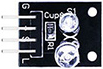
\includegraphics[angle=0, keepaspectratio=true, scale=1, width=200px, height=200px]{images/magic_cup.jpg}
    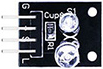
\includegraphics[angle=0, keepaspectratio=true, scale=1, width=200px, height=200px]{images/magic_cup.jpg}
    %\caption{Caption}
\end{figure}
\subsection*{Description}
This module is designed to display an optical effect. The light can 'poured' by tilting the modules as though pouring from one module to the other.

\subsection*{Pin mapping}
This pin mapping corresponds to the pins from left to right with the module pins facing towards you.
\begin{table}[H]
    \centering
    \begin{tabular}{|c|c|c|c|c|}
    \hline
    Index &Label &Type &Name &Description\\ \hline
    0 &G &Ground &GND &\\ \hline
    1 &+ & & &Unused \\ \hline
    2 &S &Digital output &D0 &Output signal from module\\ \hline
    3 &L &Analog input &A0 &Analog signal to module LED\\ \hline
    \end{tabular}
    %\caption{Caption}
    %\label{tab:my_label}
\end{table}
\subsection*{Operation}
The output voltage at the digital pin (D0) is low when the module is upright. When the module is tilted D0 will be set to high.

The LED on the module can be controlled directly setting A0 to high or applying a PWM signal for varying brightness.
%\subsection*{Code}
%\lstinputlisting[caption=test]{laser.py}